% The following is for LaTeX2e.
\documentclass[10pt]{article}
\usepackage{samplesty} % Includes the sample style file
\usepackage{epsfig}

% For algorithm elements
\usepackage{algorithm}
\usepackage[noend]{algpseudocode}

%For Neural Network Diagram
\usepackage{tikz}
\usetikzlibrary{positioning}


%plot data
\usepackage{pgfplots}
\usepackage{filecontents}
\usepackage{subcaption}




% The following is for LaTeX 2.09.
% \documentstyle[11pt,twocolumn,samplesty,epsfig]{article}

\begin{document}

\title{Deep reinforcement learning for calibration of 2D-3D registration}

\author{Eungjune Shim$^1$, Hannah Kim$^1$, Laehyun Kim$^2$, Youngjun Kim$^{1,}$\thanks{Corresponding author email: junekim@kist.re.kr}\\
$^1$Division of Bio-Medical Science \& Technology, KIST School, \\
Korea University of Science and Technology, Seoul 02792, Republic of Korea
\\ $^2$Center for Bionics, Korea Institute of Science and Technology, Seoul 02792, Republic of Korea}

\date{2017-05}
\maketitle

\begin{abstract}
The Deep Q-Learning method is a novel approach to approximate the value functions of reinforcement learning. It has been successfully applied to solve problems in robot control, elevator scheduling, and telecommunication networks. We applied this method to a simplified 2D-3D registration problem, a point-based visual servoing simulator. The simulator environment was virtually organized in 3D space: four 3D target point vectors, a 2D correct point vector, and a virtual camera are defined. For each time step, the camera moves according to the output of a neural network (Q-network), and the 3D target points are projected onto the viewport. The purpose of this simulator is to reduce 2D vector errors between target and correct point vectors. The Q-network takes the states of the current time step, selects a action, receives rewards, and updates weights. The actions are defined in six directions: the camera moves forward, backward, up, down, right, left. The state is defined as four 2D error vectors. As learning progresses, the network moves the camera to increase to probability of reducing errors. There are several advantages to using a well-trained network compared to conventional methods such as random search algorithms or Jacobian matrix estimation. While conventional methods require the computation of error variations or inverse matrix in every time step, our proposed method only requires simple network forwarding to find its solution. However, since this method used an oversimplified registration environment and camera actions, its performance was a bit awkward; but there still are a lot to improve from this approach. First, we can define each step's state with much more complex and sophisticated forms by replacing the neural network. Many convolutional neural networks have been proposed to handle 2D images. The state can be defined by simply using the virtual camera's rendered image instead of eight-digit 2D point error vectors. Second, the camera actions can be more natural and efficient by using the whole output possibility of the network and combining actions. As our proposed method shows considerable advantages over conventional methods, future work will eventually make it applicable to real 2D-3D registration processes.

\vspace*{5mm}
\noindent
{\bf Key words:}  Deep Q Learning, Reinforcement Learning, 2D-3D Registration, Visual Servoing
\end{abstract}

\newpage
\section{Introduction}
 There are various methods that use 2D features to perform in 3D space. As image processing and 3D technologies evolve and computing power increases, many related works using this approach have become possible. Some methods utilize a monoscopic camera for 3D scanning\cite{3dscanning}, camera calibration\cite{cameracalibration}, motion capture\cite{motioncapture}, or visual servoing\cite{visualservoing}, and all are using 2D features to somehow perform in 3D space. In this paper, we proposed an approach to solve 2D-3D registration problems. 2D-3D registration also uses 2D features to conduct registration in 3D. This method is largely used in the medical field. Registering 3D dicom volume obtained from computed tomography or magnetic resonance imaging to a 2D X-ray image can produce valuable information in diagnosing patient conditions. For example, when diagnosing an orthopedic patient's condition, well-aligned 3D data can be used to visualize 3D data with information that can only be obtained from X-ray images \cite{femoral, tka}.\\
 Many optimization approaches have been proposed and developed to apply to this registration task. When 2D features are simple as points, lines, or binary or faces, the Jacobian matrix estimation\cite{jacobianmatrix} method is known to be robust and is frequently used. This method extracts meaningful features from the target image, defines and calculates the error between the target and correct 2D features, and performs calibration. This method requires a considerable amount of 2D data preprocessing and feature matching in every time step, as well as large inverse matrix operations. Thus, this method is not applicable to most 2D-3D registration processes that use various 2D images such as x-ray radiographs. Many image comparison methods have been proposed, such as edge-filtering\cite{edge}, to preprocess image data for this task. Too much simplified image feature can possibly lose most of information, it might loss most of valuable information of image resulting inefficiency. For these reasons, the Jacobian matrix estimation method is unsuitable for most 2D-3D registration processes. There are also plenty of methods to define errors between 2D features \cite{validation} and optimize errors. Optimization is normally conducted using iterative methods, such as simulated annealing algorithms\cite{edge}. However, this optimization task also has limitations such as local minima or unnecessary searches.\\
 In recent years, deep learning methods have attracted interest for solving optimization problems in image or natural language processing, Most state-of-the-art methods are based on deep learning\cite{deepimage, deeplanguage}. For problems with very a large search space such as game playing or 2D-3D registration, deep reinforcement learning methods are often used. The current state-of-art reinforcement learning method is Deep Q-Network (DQN)\cite{dqn} learning proposed by \emph{DeepMind}. DQN has been successfully applied to learn and perform complex tasks such as playing Atari games\cite{ref2}. We also have chosen the DQN method to conduct 2D-3D registration. Since our method is an approach to determine whether DQN can be applied to registration problems, we made our models and problems as simple as possible. We successfully applied DQN to operate a four-point-based visual servoing simulator, recorded learning outcomes and effects, and proposed a strong future research plan based on this method.

\section{Methods}
The virtual point-based servoing simulator is composed of a camera and a plane containing four circles in a virtual 3D space. The plane normal and camera view vectors are parallel to the y-axis of the world coordinate system. Since rotation is not possible under the conditions of this simulator, the camera view vector will not be changed. In visual servoing, four feature points are normally extracted from the rendered image using image processing algorithms. Since our purpose is to test our DQN-based 2D-3D registration algorithm, we decided to skip this process. Instead, we pre-defined the 3D positions of the four feature points and extracted these to the 2D rendering viewport by unprojecting them; this has the same effect as feature detection. The simulator runs on a web browser and used a JavaScript-based \emph{WebGL} library named \emph{Three.js}.

\begin{figure}[htb]
\begin{center}
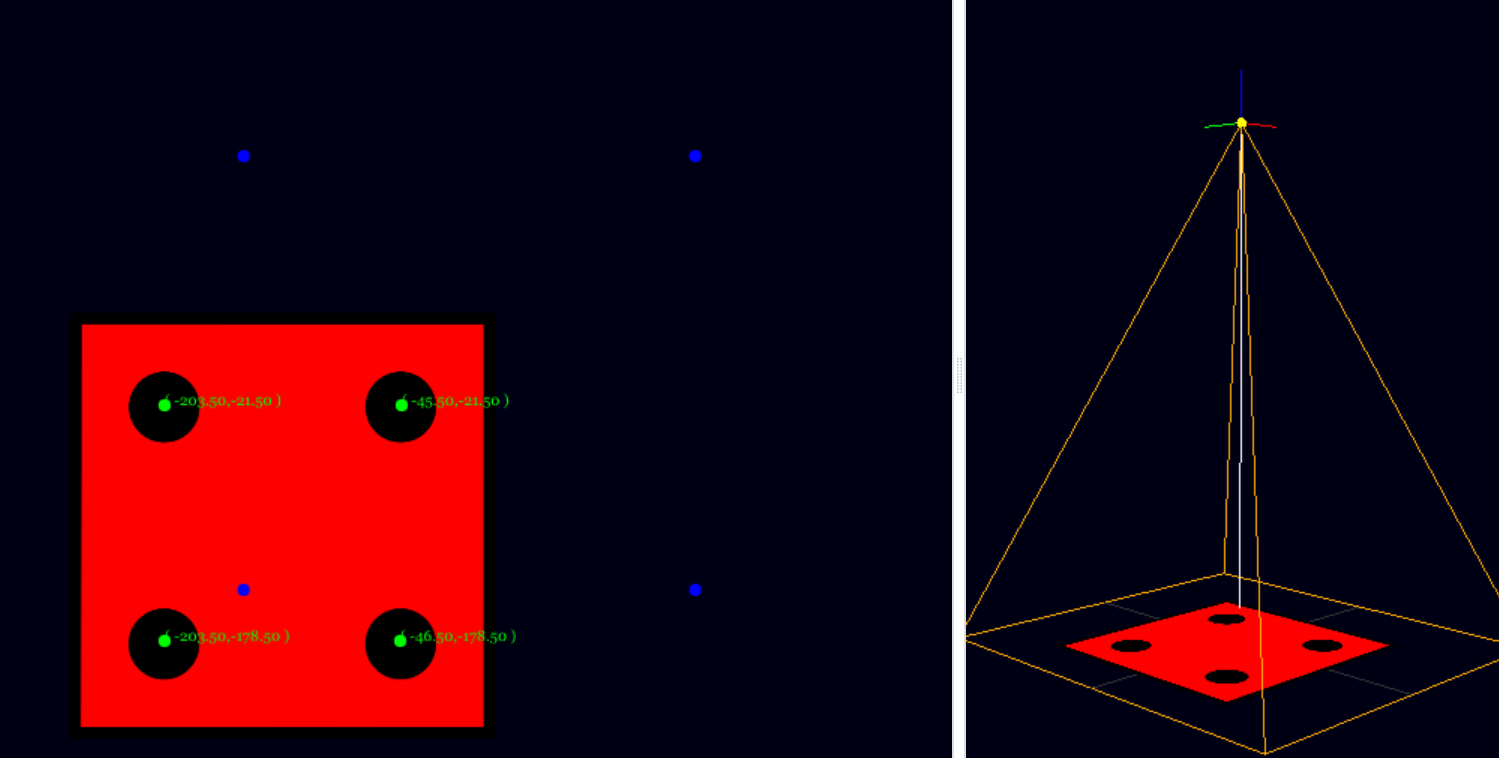
\includegraphics[width=0.8\columnwidth]{images/fig-temp1.png}
\caption{3D servoing environment: renderer image(left) and 3D objects(right)}
\label{fig1}
\end{center}
\end{figure}

DQN training is based on a Q-learning\cite{ref1} algorithm that uses a Q-network for approximating the Q-table. Experience replay and target $Q$ are also applied to our method to prevent divergence and stabilize the process. For every time step $t$, the environment $\varepsilon$, composed of states $x_t$, actions $a_t$, and rewards $r_t$ are defined. The DQN agent has a Q-network (\ref{actions}) that predicts the rewards for each action value(Equation \ref{eq1}) so that user-defined rewards can backpropagate and update weights inside the network\cite{ref2}. In our proposed method, we simply set the state as four error vectors of 2D target points and the corresponding ground truth points. The reward is given according to variations in error vector size. If the total value of the error decreases in $x_{t+1}$, the agent receives a reward valued at $1.0$; if the error increases, the reward is $-1.0$. The action $a$ moves in six directions: forward, backward, up, down, right, left. For each action, all the distance the camera move is set to $1$. The agent interacts with the simulator by selecting actions in a way that maximizes future rewards. The Q-network is composed of a simple four-layer neural network: an input layer, two fully-connected layers with 50 neurons, and a regression output layer Fig. ~\ref{fig2}.

\begin{equation}\label{eq1}
  Q(x, a ; \theta) \Rightarrow r
\end{equation}


\tikzset{%
  every neuron/.style={
    circle,
    draw,
    minimum size=0.5cm
  },
  neuron missing/.style={
    draw=none,
    scale=3,
    text height=0.333cm,
    execute at begin node=\color{black}$\vdots$
  },
}
\begin{figure}[htb]
\begin{center}
  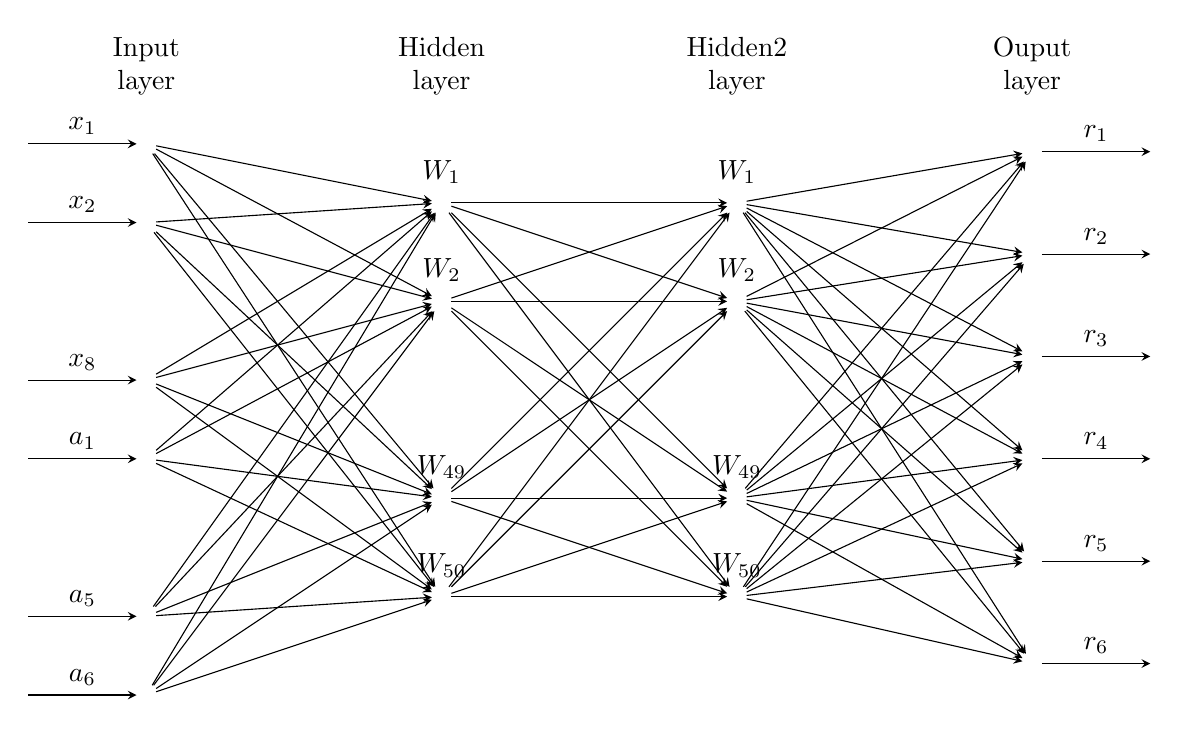
\begin{tikzpicture}[x=1.5cm, y=1.0cm, >=stealth]

 \def\layersep{2.5}
 %Input Layer
  \foreach \m/\l [count=\y] in {1,2,missing,3,4,missing,5,6}
    \node [every neuron/.try, neuron \m/.try] (input-\m) at (0*\layersep,2.5-\y) {};

%Hidden Layer 1
  \foreach \m [count=\y] in {1,2,missing,3,4}
    \node [every neuron/.try, neuron \m/.try ] (hidden-\m) at (1*\layersep,2-\y*1.25) {};

%Hidden Layer 2
  \foreach \m [count=\y] in {1,2,missing,3,4}
    \node [every neuron/.try, neuron \m/.try ] (hidden2-\m) at (2*\layersep,2-\y*1.25) {};
%Hidden Layer 1
  \foreach \m [count=\y] in {1,...,6}
    \node [every neuron/.try, neuron \m/.try ] (output-\m) at (3*\layersep,2.7-\y*1.3) {};



  \foreach \l [count=\i] in {1,2,8,1,5,6}
  {
    \ifthenelse{\i < 4}{\draw [<-] (input-\i) -- ++(-1,0) node [above, midway] {$x_{\l}$};}{\draw [<-] (input-\i) -- ++(-1,0) node [above, midway] {$a_{\l}$};}

  }


  \foreach \l [count=\i] in {1,2,49,50}
    \node [above] at (hidden-\i.north) {$W_{\l}$};

  \foreach \l [count=\i] in {1,2,49,50}
    \node [above] at (hidden2-\i.north) {$W_{\l}$};


  %Append Edge
  \foreach \l [count=\i] in {1,...,6}
    \draw [->] (output-\i) -- ++(1,0)
      node [above, midway] {$r_{\l}$};

  \foreach \i in {1,...,6}
    \foreach \j in {1,...,4}
      \draw [->] (input-\i) -- (hidden-\j);

  \foreach \i in {1,...,4}
    \foreach \j in {1,...,4}
      \draw [->] (hidden-\i) -- (hidden2-\j);

  \foreach \i in {1,...,4}
    \foreach \j in {1,...,6}
      \draw [->] (hidden2-\i) -- (output-\j);

  \foreach \l [count=\x from 0] in {Input, Hidden, Hidden2, Ouput}
    \node [align=center, above] at (\x*\layersep,2) {\l \\ layer};

  \end{tikzpicture}
\caption{Q-network in the agent. The input layer is composed of states $s$ and actions $a$. The output layer is composed of rewards}
\label{fig2}
\end{center}
\end{figure}

In the training process, the camera position is initialized randomly where all four target feature points are visible. If the error value variation $E_t$ between $x_{t+1}$ and $x_t$ is less than $10.0$, the camera is repositioned according to the camera position initialization function. After $100$ experiences are stacked, the training starts. The agent takes the state $x_t$ and decides on the action according to the DQN network policy. As learning progresses, the exploration epsilon $\epsilon$ slightly decreases, and this value causes the agent to increasingly rely on the Q-network instead of random selection when choosing the action. We set the minimum $\epsilon_{min}$ to 0.005 and when (eq??), the learning task is done. Setting $\epsilon_{min}$ to zero can make our process easily fall into the local minima. Thus, we opted to use this value to choose a random action even when running a calibration task using the trained network. The camera performs the action specified by the agent ($camera.GoTo(a_t)$). The reward $r_t$ is fixed according to $E_t$, and the agent takes the reward and updates the weights of the Q-network ($agent.Backward(r_t)$).
The epoch of the training session is set from the state when the camera is repositioned randomly until the optimal transformation that sets error values to less than $10.0$ is reached.


\begin{equation}\label{eq2}
  \epsilon \leq \epsilon_{min}
\end{equation}

 \begin{algorithm}
   \caption{DQN training process for point-based visual servoing}\label{algo1}
   \begin{algorithmic}[1]

     \State camera.RandomPosition()


     \For {$t$ in $T$}

     \State $a_t$ =  argmax(Q(s, a;$\theta$))
     \State $cam_{pos}$ = $cam_{pos}$ + $a_t$
     \State $E_t$ = Error($x_{t+1}$) - Error($x_t$)
     \If {E $\geq$ 0}
     \State $r_t$ = $1.0$
     \Else
     \State $r_t$ = -$1.0$
     \EndIf

     agent.Backward($r_t$)
     \If{$r_t$ $leq$ 10.0}
     $cam_{pos}$ = $random$
     \EndIf

     \EndFor

   \end{algorithmic}
 \end{algorithm}


\section{Results}
The duration of each epoch during training is plotted on Fig. \ref{fig3}. A total of 545 epochs and 199,108 steps were conducted to complete the training, where equation \ref{eq2} was satisfied. The average Q-learning loss was 0.7580. Fig. \ref{fig3} (a) shows that it took 492.17 s to finish epoch 0. From the second epoch, nothing exceeded 100.0 s to reach the optimal state. From epoch 76, the simulator reached the optimal states within approximately 10.0 s (Fig. \ref{fig3}, (b)). Fig. \ref{fig4} (a) shows the optimization time distribution of 30 epochs using the well-trained DQN model. It took an average 2.28 s to finish a single epoch starting from a random camera position. Each epoch's error rate variation is plotted on Fig. \ref{fig4} (b).
 Fig. \ref{fig5} shows the decreasing trend of the error rate in each epoch. As training progressed, the model not only reached its optimal state faster, but also showed less unnecessary movements, as seen in the error rate variation graphs that appeared softer in higher epochs.


\begin{figure}[htb]
\begin{center}
  \begin{tikzpicture}
      \begin{axis}[width=0.7\columnwidth, at={(0.0\columnwidth, 0)}, name = a,
          x label style={ at={(ticklabel* cs:0.5)},anchor=east},
          y label style={ at={(ticklabel* cs:0.5)},anchor=south},
          xlabel={ epochs },
          ylabel={ time ($seconds$) }]
          \addplot[red] table [x=episodes, y=time, col sep=comma] {data/progress.csv};
      \end{axis}
      %subplot
      \node[above] at (a.north) {(a)};

      \begin{axis}[width=0.5\columnwidth, at={(0.15\columnwidth, 2 cm)}, name = b]
          \addplot[only marks] table [x=episodes, y=time, col sep=comma] {data/progress2.csv};
      \end{axis}
      \node[above] at (b.north) {(b) From epoch 78};
  \end{tikzpicture}
\caption{Searching time during learning progress}
\label{fig3}
\end{center}\end{figure}


\begin{figure}[htb]
\begin{center}
  \begin{tikzpicture}
      \begin{axis}[width=0.5\columnwidth, at={(-0.1\columnwidth, 0)}, name = a,
          x label style={ at={(ticklabel* cs:0.5)},anchor=east},
          y label style={ at={(ticklabel* cs:0.5)},anchor=south},
          xlabel={ $epochs$ },
          ylabel={ time ($seconds$) }]
          \addplot[only marks] table [y=time, col sep=comma] {data/well-trained/progress.csv};
      \end{axis}
      \node[above] at (a.north) {(a)};

      \begin{axis}[width=0.5\columnwidth, at={(0.5\columnwidth, 0)}, name = b,
        x label style={ at={(ticklabel* cs:0.5)},anchor=east},
        y label style={ at={(ticklabel* cs:0.5)},anchor=south},
        xlabel={ iterations },
        ylabel={ error rates }]
        \foreach \i in {510,..., 540}
          \addplot[red] table [x=iterations, y=error, col sep=comma] {data/well-trained/out_\i.csv};
      \end{axis}
      \node[above] at (b.north) {(b)};
  \end{tikzpicture}
\caption{Well-trained network calibration error variation}
\label{fig4}
\end{center}\end{figure}



\def\ysep{5.0}
\def\xsep{0.35}
\def\wid{0.40\columnwidth}
\begin{figure}[htb]
\begin{center}
  \begin{tikzpicture}
    \begin{axis}[width=\wid, at={(0.0, -0.0)}, name=graph1, ymax = 200]
        \addplot[blue] table [x=iterations, y=error, col sep=comma] {data/out_0.csv};
    \end{axis}

    \begin{axis}[width=\wid, at={(\xsep\columnwidth, -0.0)}, name=graph2, ymax = 200]
      \foreach \i in {1,...,10}
        \addplot[blue] table [x=iterations, y=error, col sep=comma] {data/out_\i.csv};
    \end{axis}

    \begin{axis}[width=\wid, at={(\xsep*2\columnwidth, -0.0)}, name=graph3, ymax = 200]
      \foreach \i in {11,...,110}
        \addplot[blue] table [x=iterations, y=error, col sep=comma] {data/out_\i.csv};
    \end{axis}



    \begin{axis}[width=\wid, at={(0.0\columnwidth, -\ysep cm)}, name=graph4, ymax = 200]
      \foreach \i in {111,...,200}
        \addplot[blue] table [x=iterations, y=error, col sep=comma] {data/out_\i.csv};
    \end{axis}
    %
    %
    % \begin{axis}[width=0.4\columnwidth, at={(\xsep\columnwidth, -\ysep cm)}, name=graph5, ymax = 200]
    %   \foreach \i in {201,...,250}
    %     \addplot[blue] table [x=iterations, y=error, col sep=comma] {data/out_\i.csv};
    % \end{axis}
    %
    %
    % \begin{axis}[width=0.4\columnwidth, at={(\xsep*2\columnwidth, -\ysep cm)}, name=graph6, ymax = 200]
    %   \foreach \i in {251,...,300}
    %     \addplot[blue] table [x=iterations, y=error, col sep=comma] {data/out_\i.csv};
    % \end{axis}
    %
    %
    %
    %
    % \begin{axis}[width=0.4\columnwidth, at={(0.0\columnwidth, -\ysep*2 cm)}, name=graph7, ymax = 200]
    %   \foreach \i in {301,...,350}
    %     \addplot[blue] table [x=iterations, y=error, col sep=comma] {data/out_\i.csv};
    % \end{axis}
    %

    \begin{axis}[width=\wid, at={(\xsep\columnwidth, -\ysep cm)}, name=graph5, ymax = 200]
      \foreach \i in {351,...,400}
        \addplot[blue] table [x=iterations, y=error, col sep=comma] {data/out_\i.csv};
    \end{axis}


    % \begin{axis}[width=0.4\columnwidth, at={(\xsep*2\columnwidth, -\ysep*2 cm)}, name=graph9, ymax = 200]
    %   \foreach \i in {401,...,450}
    %     \addplot[blue] table [x=iterations, y=error, col sep=comma] {data/out_\i.csv};
    % \end{axis}
    %



    %
    % \begin{axis}[width=0.4\columnwidth, at={(0.0\columnwidth, -\ysep*3 cm)}, name=graph10, ymax = 200]
    %   \foreach \i in {451,...,500}
    %     \addplot[blue] table [x=iterations, y=error, col sep=comma] {data/out_\i.csv};
    % \end{axis}
    %
    %
    % \begin{axis}[width=0.4\columnwidth, at={(\xsep\columnwidth, -\ysep*3 cm)}, name=graph11, ymax = 200]
    %   \foreach \i in {501,...,540}
    %     \addplot[blue] table [x=iterations, y=error, col sep=comma] {data/out_\i.csv};
    % \end{axis}


    \begin{axis}[width=0.4\columnwidth, at={(\xsep*2\columnwidth, -\ysep cm)}, name=graph6, ymax = 200]
      \foreach \i in {541,...,545}
        \addplot[red] table [x=iterations, y=error, col sep=comma] {data/out_\i.csv};
    \end{axis}


    %Add Description
    \foreach \l [count=\i] in {0,1--10,11--110,111--200, 351--400, 541--545(last Epoch)}{
      \node[above] at (graph\i.north) {Epoch \l};}

  \end{tikzpicture}
\caption{Error rate variation. Error rate(y-axis), and iterations(x-axis)}
\label{fig5}
\end{center}\end{figure}



\section{Discussion}
 Our proposed DQN model was trained using 2D feature vector error as the state $x$ and selected the correct action $a = argmax(Q(s,a;\theta))$ for the visual servoing camera in 3D space. Under our DQN policy, the model finished training after 545 epochs. The well-trained model can conduct registration from a random position to the optimal state within an average of 2.28 s. The visualized camera moved smoothly with almost no unnecessary movement. Compared to conventional methods such as random search tree algorithms or Jacobian matrix estimation, our proposed method has several advantages. First, the amount of calculations is greatly reduced. Both conventional methods require the calculation of error variations in every time step. Furthermore, the Jacobian matrix estimation method requires calculation of the inverse (or pseudoinverse) matrix every time. Random tree search algorithms such as simulated annealing can easily to fall into the local minima, and there are also excessive unnecessary movements during registration. The DQN method requires such calculations only during training. Once training is completed, it no longer requires complex computations and shows efficient servoing movement. Second, the proposed method is very easy to implement. Once the form of the network, environment, actions, rewards, and some parameters are configured, difficult tasks are eliminated except waiting for the agent to be trained.

 However, there are currently several limitations that need to be addressed. First, camera movement is somewhat inefficient because the direction and range of movement is fixed to six actions. The Jacobian matrix estimation method can generate an all-round 3D translation and rotation vector, and currently has much smoother motion during registration. Since all the distance the camera move is $1$, it is also inefficient in terms of utilization of error sizes. Second, state $x_t$ is too simple to apply to real 2D-3D registrations. Although our current method defined $x_t$ as four 2D point vector errors, real 2D-3D registration has larger and more complex features that need to be used to define current state.

  Most of these limitations can be resolved in the future works. The camera movement problem can be solved by combining actions. Instead of choosing a single action predicted by $argmax(Q(s, a; \theta ))$, we can use the whole values in the output layer of the Q-network, and add the action vectors multiplied by the corresponding predicted reward values. This can provide a higher degree of freedom to camera motion. The addition of rotational action is also necessary to perform complicated 2D-3D registration. A more sophisticated form of state $x$ can also be easily defined. This is the greatest advantage of using DQN rather than other methods. Compared to the Jacobian matrix estimation method, as the features of the input state become more complicated, the computation and complexity of deciding the proper action becomes exponentially more difficult.
  This method can use a convolutional neural network (CNN) that can self-study the feature information of input images. This method is also extremely easy to implement and can provide good results. Many DQN methods have been successfully applied to playing games that use rendered game images as the input state and deep CNN as its Q-networks\cite{ref2}. Setting stochastic rewards can also efficiently utilize the size of error variations, and reduce registration time. To summarize, our future DQN model uses a deep CNN for its value network. It takes the rendered image of each time step as the input state, predicts actions, and performs registration by combining the whole output Q-network layer. The reward for this registration method could be the root mean square error between the pre-defined optimal transformation and current transformation. This model is expected to perform very well compared to most conventional methods using rigid single-view 2D-3D registration



\section{Conclusion}

We have proposed and developed a DQN method for 2D-3D registration. This method was successfully applied to optimize and solve a point-based visual servoing simulator. Since this simulator takes 2D feature states to perform in 3D, it can be regarded as a very simplified 2D-3D registration simulator. Although this is a simplified problem, the strength of the proposed approach is its ability to solve similar but more complex problems compared to conventional registration methods. For example, the Jacobian matrix estimation method requires exponential computations and high difficulty as the problem becomes more complicated. Most search algorithms such as simulated annealing and heel climbing methods for optimizing 2D-3D registration require calculation of the similarity between two states. As the complexity of two states increases, the amount of computations also increases. Although the well-trained DQN model only forwards input states to the network to determine proper actions, its inherent advantages will enable the resolution of most limitations in the near future, when this approach is applied to higher-order 2D-3D registration problems.


\section*{Acknowledgement}
This research was supported by the KIST institutional program (2E26880, 2V05430).


\newpage
\bibliographystyle{elsarticle-num}
\bibliography{references}


\end{document}
